\documentclass{acm_proc_article-sp}
%\documentclass{sig-alternate}

% Set letter paper size:
%\setlength{\paperheight}{11in}
%\setlength{\paperwidth}{8.5in}

\usepackage{authblk}
%\renewcommand\Authfont{\small}
%\renewcommand\Affilfont{\itshape\footnotesize}

\usepackage{times,amsmath,epsfig}
\usepackage[hyphens]{url}
\usepackage[pagebackref=true]{hyperref}
%\usepackage[hang,raggedright]{subfig}
%\usepackage[font=footnotesize]{subfig}
\usepackage{subfig}
\usepackage{amsmath, graphicx}
%\usepackage{multiFloats}
\usepackage{url}
\usepackage{verbatim}
\usepackage{amssymb,amsmath}
\usepackage{alltt}
%\usepackage{pslatex}
%\usepackage[all]{xy}
\usepackage{color}
\usepackage{listings}

\newcommand\F[1]{\textcolor{red}{F: #1}}
\newcommand\K[1]{\textcolor{red}{K: #1}}
\newcommand\R[1]{\textcolor{red}{R: #1}}

\begin{document}
%\sloppy
%\thispagestyle{empty}
\title{\textbf{Information Loss During Size Reduction Depending On Structure Scale}}

\author[1]{Laurens Bogaardt}
\author[1]{Romulo Goncalves}
\author[2]{Raul Zurita-Milla}
\author[2,3]{Emma Izquierdo-Verdiguier}

\affil[1]{NLeSC Amsterdam, The Netherlands \vspace{1pt} \{\emph{\{l.bogaardt, r.goncalves\}@esciencecenter.nl}\}}%, o.rubi\}@esciencecenter.nl}\}}
\affil[2]{Faculty of Geo-Information Science and Earth Observation (ITC), University of Twente, the Netherlands \vspace{10pt} \{\{\emph{\{r.zurita-milla,e.izquierdoverdiguier\}@utwente.nl}\}\}}
\affil[3]{Image Processing Laboratory (IPL), Universitat de Valencia, Spain}

\date{} % <--- leave date empty
\maketitle\thispagestyle{empty} %% <-- you need this for the first page

\begin{abstract}
The analysis of large datasets can be time consuming and costly. Often, techniques exist to arrive at the same output, or at a close approximation, which require far less effort. This article looks at several such techniques and at the inherent scale of the structure within the data. When the values of a dataset vary slowly, e.g. in a spatial field of temperature over a country, there is a high level of auto correlation and the structure of the field has a large scale. Datasets need not have a high resolution to describe such fields faithfullly. Using generated \textit{Gaussian Random Fields} with various levels of spatial auto correlation, we examine several exact and approximate analysis techniques. Our aim is to outline when certain techniques can be useful and to find a relation between performance and the scale of the structure described by the input datasets.
\end{abstract}

\section{Introduction}
\label{sec:Introduction}

General introduction about CCA, MCA and phenology~\cite{Eshel2011, Storch1999}.
%Eshel:
% - when neighboring data points are not entirely independent of one another, there is some redundancy in the time series. 

\subsection{Gaussian Random Spatial Field}
\label{sec:Introduction Gaussian Random Spatial Field}

In order to compare analysis techniques and to find the relation between performance and the structrue scale, we need to be able to generate fields which resemble fields often encountered in real-world applications. In particular, the field we will concern ourselves with need to have some amount randomness and some level of spatial auto correlation. Gaussian Random Fields are particularly useful, as their structure scale can be captured in a single parameter. The power spectrum of such a field follows the power law described in equation~\ref{eq:powerLaw} where $k$ is the wave number and $\alpha$ the parameter which controls the level of auto correlation. For 2D spatial fields, rotational invariance is assumed, such that $k$ can be substituted by $||k||$.
\begin{equation}
\label{eq:powerLaw}
f = k^{-\alpha}
\end{equation}

In spatial data analysis, other measures of auto correlation are often used~\cite{Eshel2011, Storch1999}. These include Moran's I and the $\Gamma$ index~\cite{Moran1950, Hubert1981, PySAL}.

The singular values of a zero-mean matrix represent the amount of variance in the original dataset explained by the associated singular vector. For Gaussian Random Fields, depending on the scale parameter $\alpha$, the singular values decay quickly. One can try to fit a power law and estimate the exponent, which we'll call $\beta$. 

The $\alpha$ is a measure of the spatial autocorrelation of the field. In particular, fields with large scale structure have a more negative $\alpha$. Additionally, the size of the singular values can be plotted. This is related to the power spectrum and will also provide information about the scale of the structure in the field. Finally, there are other measures of spatial autocorrelation. These include the Gamma Index and Moran's I. The Python module pysal contains functions to calculate these values. We will include them for each plot.

\begin{figure}[h]
\begin{center}
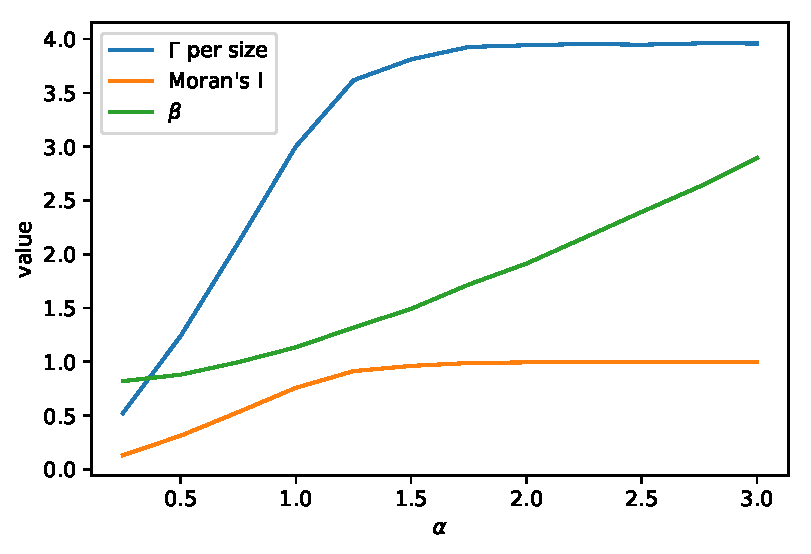
\includegraphics[width=0.8\columnwidth]{Results/plotGammaAndMoransIAndBeta.pdf}
\caption[Small caption]{Caption}
\label{fig:plotGammaAndMoransIAndBeta}
\end{center}
\end{figure}
When $\alpha$ is less negative, the Gaussian Random Field has smaller scale structure. It is closer to randomness and has less autocorrelation. As expected, this can be seen in the two measures of autocorrelation, which are now smaller.

\subsection{Gaussian Random Spatial-Temporal Field}
\label{sec:Introduction Gaussian Random Spatial-Temporal Field}

In many real-world applications, the analysis of a field does not only involve a single time snapshot. In fact, it often includes data over multiple weeks, months or years, where the field over the entire time period does not change drastically. Just as there is spatial autocorrelation, there is temporal autocorrelation. In principle, there can be a different level of correlation over time than over space. However, for simplicity, we are using the same $\alpha$ determine the level of autocorrelation in all dimensions.

Lorem Ipsum is simply dummy text of the printing and typesetting industry. Lorem Ipsum has been the industry's standard dummy text ever since the 1500s, when an unknown printer took a galley of type and scrambled it to make a type specimen book. It has survived not only five centuries, but also the leap into electronic typesetting, remaining essentially unchanged. It was popularised in the 1960s with the release of Letraset sheets containing Lorem Ipsum passages, and more recently with desktop publishing software like Aldus PageMaker including versions of Lorem Ipsum.

\subsection{CCA and MCA Analyses}
\label{sec:Introduction CCA and MCA Analyses}

In an MCA, modes are found where the left- and the right-field covary maximally~\cite{Bretherton1992}. One technique to find these modes is to perform an SVD on the product of the datasets. That is why the term SVD is often used synonymously with MCA.
In an CCA, modes are found where the left- and the right-field correlate maximally. In practice, the datasets are first standardized before multiplied and decomposed. MCA and CCA are very much related, but the resulting modes and vectors need not be the same~\cite{Bretherton1992}.
In a PCA, the first and the second dataset are identical. Whether to maximize the covariance or the correlation depends on whether the units of each vector is the same.

\section{Techniques}
\label{Techniques}

This section will discuss four techniques to analyse large datasets efficiently using SVD.

\subsection{Exact Norm Difference via SVD}
\label{sec:Techniques Exact Norm Difference via SVD}

In real-world application, one often wants to find the norm of the difference between two fields. This can be done by subtracting one matrix from the other and calculating the norm. However, for large matrices, this can be inefficient. Performing an SVD of both matrices can reduce the internal calculations.

Let $|| \cdot ||$ indicate the Frobenius norm, $\left\langle \cdot \right\rangle$ the Frobenius inner product and the $\circ$ operator the Hadamard product, then the norm of the difference between matrices $A$ and $B$ is given by equation~\ref{eq:normDifferenceFromUSVs}.
\begin{equation}
\label{eq:normDifferenceFromUSVs}
\begin{split}
||A-B||^{2} & = ||A||^{2} + ||B||^{2} - 2 \left\langle A, B \right\rangle \\
& = s_{1} s_{1}^{T} +  s_{2} s_{2}^{T} - 2 s_{1} \left( U_{1}^{T} U_{2} \circ V_{1}^{T} V_{2} \right) s_{2}^{T}
\end{split}
\end{equation}

Figure~\ref{fig:normDifferenceFromUSVs} shows that this procedure can determine the norm in an efficient manner, provided the number of singular values is small. The result is mathematically identical to the full calculation, which means that any error will be of the order of machine-precision.

\begin{figure}[h]
\begin{center}
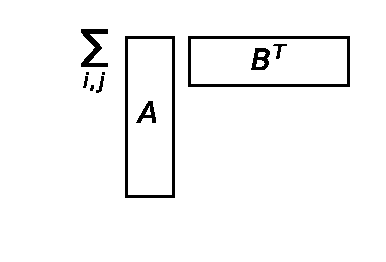
\includegraphics[width=\columnwidth]{Results/normDifferenceFromUSVs.pdf}
\caption[Small caption]{Caption}
\label{fig:normDifferenceFromUSVs}
\end{center}
\end{figure}
For very large datasets, the SVDs may be obtained using a random algorithm reviewed extensively in an article by Halko et al.~\cite{Halko2011}. The number of singular values will then be truncated to the $k$ largest values. In section~\ref{sec:Techniques Approximate SVD via Dimensionality Reduction}, we will also apply this technique to our generated fields. In this case, the resulting norm wil no longer be exact, but the error can be made arbitrarily small by adjusting $k$.

\subsection{Exact SVD via QR Decomposition}
\label{sec:Techniques Exact SVD via QR Decomposition}

The techniques discussed here are by no means novel~\cite{Golub1970, Bjorck1973, Chan1982, Tygert2017}.

In real-world applications, one often wants to find the relation between two fields. Analyses such as the MCA and CCA discussed in section~\ref{sec:Introduction CCA and MCA Analyses} rely on performing an SVD of the cross-covariance or cross-correlation matrix of the two fields. In particular, the two input datasets often have the various gridpointa as rows and will have the sample of recorded values over time as columns. Multiplying these gives the cross-correlation matrix. However, for highly rectangular matrices, when there are many spatial gridpoint but few temporal samples, the resulting cross-correlation matrix is inefficiently large. The qrProductSVD function can take such input data and perform an SVD in an efficient manner. The result is mathematically identical to the full SVD, which means that the difference will be at machine-precision.

\begin{figure}[h]
\begin{center}
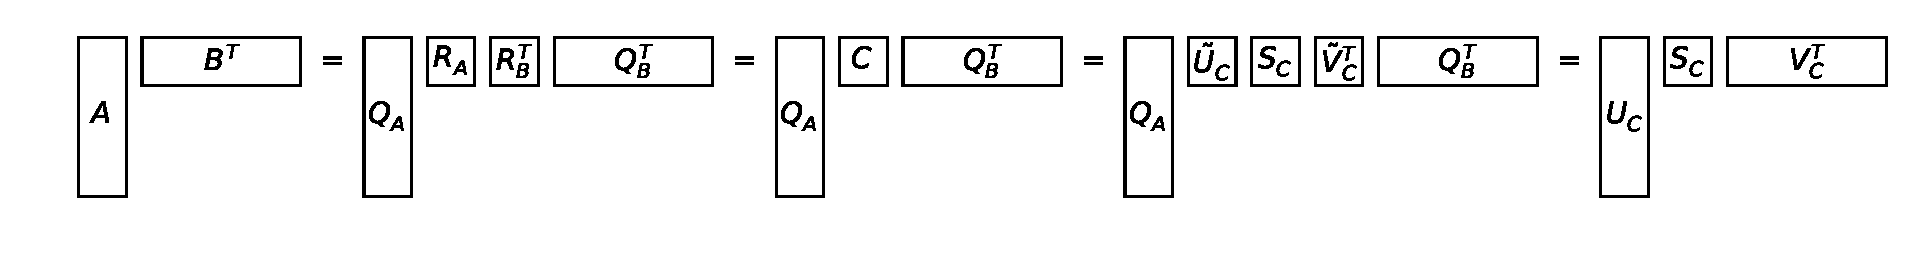
\includegraphics[width=\columnwidth]{Results/qrProductSVD.pdf}
\caption[Small caption]{Caption}
\label{fig:qrProductSVD}
\end{center}
\end{figure}
\subsection{Approximate SVD via Spatial Coarsening}
\label{sec:Techniques Approximate SVD via Spatial Coarsening}

Although the qrProductSVD function works well for two rectangular matrices, sometimes the input data is large and square. Performing an SVD on such a large dataset will be time consuming and, perhaps, inefficient given the desired level of precision. When a field have large scale structure, the values of neighbouring cells do not change drastically. This is what autocorrelation means. As such, perhaps neighbouring cells can be averaged together to produce a smaller dataset which still faithfully describes the original field. The matrixToGrid function can cut a matrix into multiple smaller sections.

\begin{figure}[h]
\begin{center}
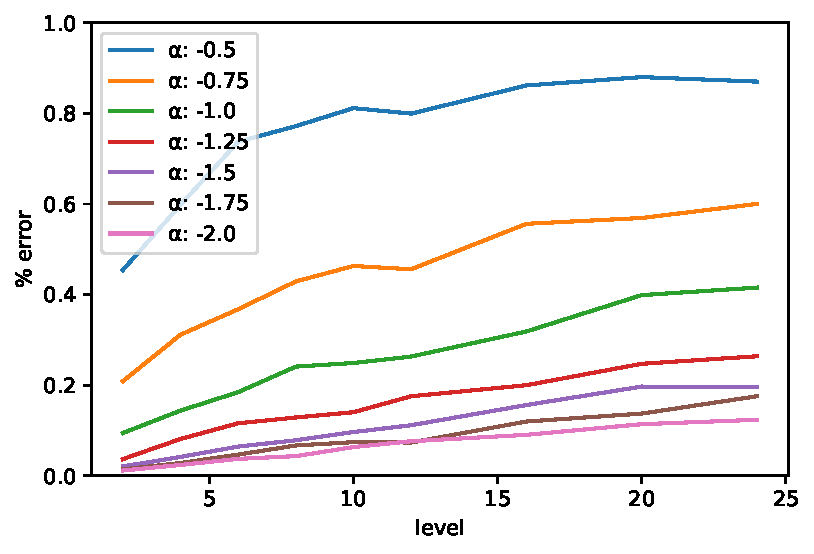
\includegraphics[width=0.8\columnwidth]{Results/plotSingleSpatialFieldViaCoarsening.pdf}
\caption[Small caption]{Caption}
\label{fig:plotSingleSpatialFieldViaCoarsening}
\end{center}
\end{figure}
The testProductSpatialTemporalFieldsViaCoarsening function determines the percentage of the information lost in a coarsening process for matrices of various sizes and $\alpha$'s, and at various levels of coarsening. The two input matrices used here are similar, as they are generated by the same Gaussian Random Process. Therefore, they will correlate highly and the bases in which they are best described will be similar. In principle, any two datasets can be analysed and the amount of information lost during the coarsening process will likely depend on the similarity between the two datasets. This is one aspect which we do not cover here and leave for further research.

Due to the multiplication step in this analysis, the typical error due to coarsening is larger than before. As before, $\alpha$ plays an important part, with more negative $\alpha$'s leading to a less dramatic loss in information due to coarsening.

\begin{figure}[h]
\begin{center}
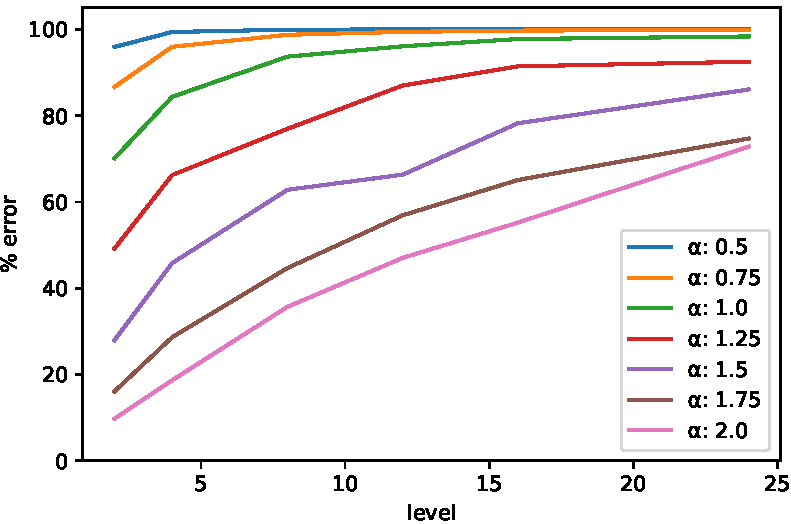
\includegraphics[width=0.8\columnwidth]{Results/plotProductSpatialTemporalFieldsViaCoarsening.pdf}
\caption[Small caption]{Caption}
\label{fig:plotProductSpatialTemporalFieldsViaCoarsening}
\end{center}
\end{figure}
The additional benefit of coarsening is that data collection can be optimised.

\subsection{Approximate SVD via Dimensionality Reduction}
\label{sec:Techniques Approximate SVD via Dimensionality Reduction}
%Halko:
%-For a matrix that is too large to fit in fast memory, the randomized techniques require only a constant number of passes over the data, as opposed to O(k) passes for classical algorithms. In fact, it is sometimes possible to perform matrix approximation with a single pass over the data
%-Compared with standard deterministic algorithms, the randomized methods are often faster and—perhaps surprisingly—more robust.
%-low-rank matrix approximations
%-The inner dimension k is sometimes called the numerical rank of the matrix. When the numerical rank is much smaller than either dimension m or n, a factorization such as (1.1) allows the matrix to be stored inexpensively and to be multiplied rapidly with vectors or other matrices
%-A basic method in statistics and data mining is to compute the direction s of maximal variance in vector-valued data by performing principal component analysis (PCA) on the data matrix.
%-Another standard technique in data analysis is to perform low-dimensional embedding of data under the assumption that there are fewer degrees of freedom than the ambient dimension would suggest
%-the failure probability decreases superexponentially with the oversampling parameter p
%~\cite{Li2016}
The spatial coarsening process is intuitive and easy to implement. It is not, however, the most efficient way to reduce the size of a dataset. Dimensionality reduction refers to discarding modes which contribute little to the variance in a dataset. An SVD is precisely the procedure used to find modes which explain as much variance as possible. Discarding the smallest singular values/vectors is, therefore, the most efficient form of dimensionality reduction. Performing an SVD on a large dataset, however, is computationally costly. The Randomised Dimensionality Reduction process is far more efficient.

The reduceSizeRandomisedSquare function reduces the input matrix to a smaller square matrix of l by l. It also gives two projection matrices which can bring the rows and columns of this smaller matrix back to the bases of the original input. To make the result more precise, the procedure can be repeated multiple times. The parameter i indicates how many loops are performed.

\begin{figure}[h]
\begin{center}
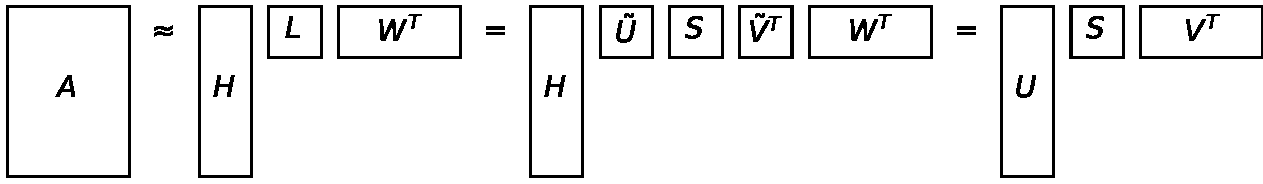
\includegraphics[width=\columnwidth]{Results/reduceSizeRandomisedSquare.pdf}
\caption[Small caption]{Caption}
\label{fig:reduceSizeRandomisedSquare}
\end{center}
\end{figure}
As seen, it is possible for some fields to be represented by matrices of much smaller sizes without losing any substantial amount of information. This is obvious when one realises the singular modes which are removed during the reduction are the smallest ones, described by the tail-end of the power law. In the review article by Halko, Martinsson and Tropp on randomised dimensionality reduction, it is suggested to oversample the reduction. This is because the error introduced in the process is of the same order as the size of the last sampled singular value. If one is interested in the k dominant modes, reducing to a k + l, for some small l, rank approximation will ensure the first k modes are approximated quite well. Indeed, as seen below, the more modes one is interested in, the larger the difference compared with the original matrix.

The Randomised Dimensionality Reduction process can also be applied to the CCA or MCA analysis of two spatial-temporal fields. Similar to the QR Product SVD, it has the advantage that the SVD is applied to a small l x l matrix. The result will be an approximation, but, as we will see, can be close to the real solution.

\begin{figure}[h]
\begin{center}
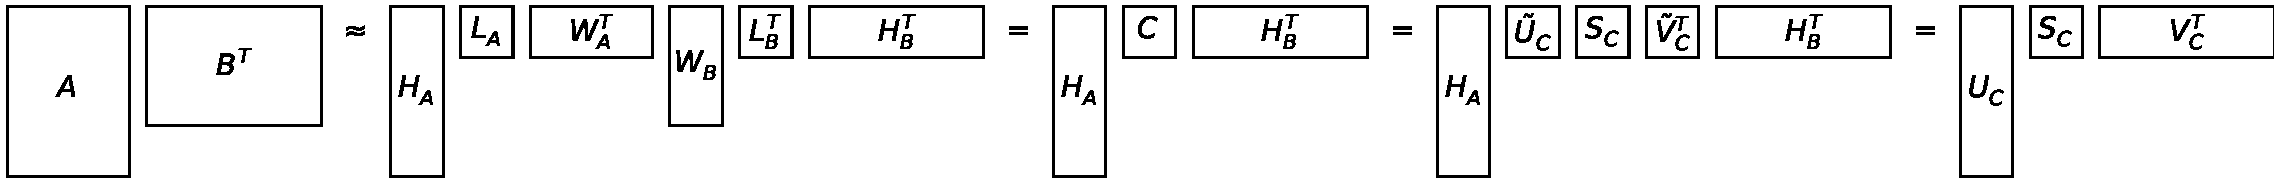
\includegraphics[width=\columnwidth]{Results/randomisedSquareProductSVD.pdf}
\caption[Small caption]{Caption}
\label{fig:randomisedSquareProductSVD}
\end{center}
\end{figure}
To see the effect of dimensionality reduction on such a matrix product, let's generate two Gaussian Random Fields and plot their corss-correlation matrix together with a reduced version. To determine precisely how much information is lost during the reduction, we should look at the variance of the datasets. The norm of the difference between the reduced matrix and the original is the amount of information lost in the reduction process.

\begin{figure}[h]
\begin{center}
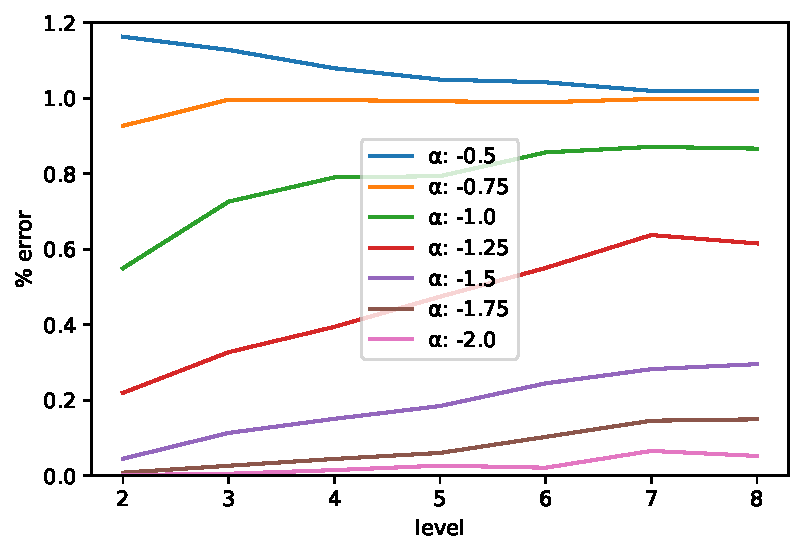
\includegraphics[width=0.8\columnwidth]{Results/plotRandomisedSizeReducedMatrixProduct.pdf}
\caption[Small caption]{Caption}
\label{fig:plotRandomisedSizeReducedMatrixProduct}
\end{center}
\end{figure}
The testRandomisedSizeReducedMatrixProduct function determines the percentage of the information lost in a reduction process for matrices of various sizes and $\alpha$'s, and at various levels of reduction. The two input matrices used here are similar, as they are generated by the same Gaussian Random Process. Therefore, they will correlate highly and the bases in which they are best described will be similar. In principle, any two datasets can be analysed and the amount of information lost during the coarsening process will likely depend on the similarity between the two datasets. This is one aspect which we do not cover here and leave for further research.

Due to the multiplication step in this analysis, the typical error due to reduction is larger than before. There is an affect of temporal size on the information loss. The randomisedSquareProductSVD function is especially useful for square input matrices. To be able to do the comparisons with the full SVD quickly, we use rectangular matrices here. The larger the temporal size, the more square the input matrices. As before, the scale of the structure of the field influences the information loss. The effect in this case can be quite dramatic. Especially for more negative $\alpha$, this procedure performs much better than the coarsening procedure.

Note that, unlike the coarsening procedure, the reduction is not applied on each time-slice of the spatial field, but rather on the spatially-flattened time-series. Therefore, the level of spatial auto correlation may not be as important as the level of temporal auto correlation. The proper analysis of this is left for further research.

The reduction of the number of dimensions of each input dataset is actually advised by some researchers, as a method to filter out noise~\cite{Barnett1987}. Especially when the number of temporal samples is small, outliers and random fluctuations could affect the result~\cite{Bretherton1992}. This is because any statistical analysis will choose its regression-coefficients so as to optimize the fit. It may occur that two noise-vectors in the two fields coincidentally covary. In a CCA, where the fields are standardized, this resulting mode may appear important even though it stems from noise. In an MCA, the variance of the noise will be low, so the chance that it will appear as an important mode is less~\cite{Bretherton1992}. One method of finding the right level of filtering is by bootstrapping/cross-validating the results~\cite{Livezey1999}.

\section{Applications}
\label{Applications}

Lorem Ipsum is simply dummy text of the printing and typesetting industry. Lorem Ipsum has been the industry's standard dummy text ever since the 1500s, when an unknown printer took a galley of type and scrambled it to make a type specimen book. It has survived not only five centuries, but also the leap into electronic typesetting, remaining essentially unchanged. It was popularised in the 1960s with the release of Letraset sheets containing Lorem Ipsum passages, and more recently with desktop publishing software like Aldus PageMaker including versions of Lorem Ipsum.

\subsection{Approximate SVD via Spatial Coarsening}
\label{sec:Applications Approximate SVD via Spatial Coarsening}

Lorem Ipsum is simply dummy text of the printing and typesetting industry. Lorem Ipsum has been the industry's standard dummy text ever since the 1500s, when an unknown printer took a galley of type and scrambled it to make a type specimen book. It has survived not only five centuries, but also the leap into electronic typesetting, remaining essentially unchanged. It was popularised in the 1960s with the release of Letraset sheets containing Lorem Ipsum passages, and more recently with desktop publishing software like Aldus PageMaker including versions of Lorem Ipsum.

\subsection{Approximate SVD via Dimensionality Reduction}
\label{sec:Applications Approximate SVD via Dimensionality Reduction}

Lorem Ipsum is simply dummy text of the printing and typesetting industry. Lorem Ipsum has been the industry's standard dummy text ever since the 1500s, when an unknown printer took a galley of type and scrambled it to make a type specimen book. It has survived not only five centuries, but also the leap into electronic typesetting, remaining essentially unchanged. It was popularised in the 1960s with the release of Letraset sheets containing Lorem Ipsum passages, and more recently with desktop publishing software like Aldus PageMaker including versions of Lorem Ipsum.

\section{Further Questions}
\label{Further Questions}

It may be interesting to extend this research to fields other than the Gaussian Random Field. This type was chosen because its structure scale can be captured in a single parameter $\alpha$. In many applications, however, the dataset does not resemble such a Gaussian Random Field.

Additionally, it would be an improvement to relax the assumption that the auto-correlation in the time direction is similar to that in the spatial directions. In fact, it may even be more realistic to have different levels of auto correlation in the $x$ and in the $y$ direction.

Can similar tricks be used to the generalised MCA/CCA analysis, where the input to the SVD in a concatenation of multiple cross-correlation matrices~\cite{Carroll1970, Kettenring1971}?

Can the dimensionality reduction be applied to the spatial part of the spatial-temporal fields, before it is flattened?

{
\footnotesize
\bibliographystyle{abbrv}
%\phantomsection
%\label{sec:Bibliography}
\bibliography{Bibliography}
}

\end{document}
